\documentclass[a4paper,english]{article}
\usepackage[utf8]{inputenc}
\usepackage[T1]{fontenc,url}
\usepackage{babel,textcomp}
\usepackage{enumitem}
\usepackage{graphicx}
\usepackage{amsmath}
\usepackage{float}
\usepackage{verbatim}
\usepackage{subfig}
\usepackage{bm}
\usepackage{mathtools}
\usepackage{dsfont}
\usepackage{gensymb}
\usepackage{multirow}
\usepackage{booktabs}
\renewcommand{\arraystretch}{1.2}
\floatstyle{plaintop}
\restylefloat{table}
\urlstyle{sf}
\def\doubleunderline#1{\underline{\underline{#1}}}
\def\unit#1{\vec{\hat{#1}}}
\renewcommand\vec{\mathbf}
\newcommand\Nabla{\boldsymbol{\nabla}}
\newcommand\norm[1]{\left\lvert#1\right\rvert}
\newcommand\Res[1]{\text{Res}\left(#1\right)}
\let\originalleft\left
\let\originalright\right
\renewcommand{\left}{\mathopen{}\mathclose\bgroup\originalleft}
\renewcommand{\right}{\aftergroup\egroup\originalright}
\makeatletter
\newcommand{\RN}[1]{\expandafter\@slowromancap\romannumeral #1@}
\makeatother
\allowdisplaybreaks
\title{FYS4150 - Project 1: Differential Equations and Linear Algebra}
\author{Tore Klungland (torekl)}
\begin{document}
\maketitle
\begin{abstract}
  This project explores three different linear algebra-based algorithms for solving Poisson's equation in one dimension: One using LU decomposition and two which use the fact that the matrix equations in question contain tridiagonal matrices. Of the latter, one is a general algorithm which may be used to solve matrix equations with any tridiagonal matrix, while the other is specialized to the particular matrix which arises in this problem. A second-order approximation for the second derivative was used, meaning that the relative error in the results should be proportional to $h^2$ where $h$ is the step size. The results show that this is indeed the case for all algorithms, for relatively large $h$; for a number of grid points $n>10^6$ the step size becomes so small that round-off errors become significant. This effect was lessened somewhat for the specialized tridiagonal algorithm as some values were calculated from a closed-form expression here, instead of using repeated floating point operations as in the other methods. \par
  The efficiency of these methods (i.e. the CPU time used) was also compared; here the results showed that the tridiagonal matrix algorithms have a CPU time roughly proportional to the number of integration points $n$, and slightly less for the specialized version than the general one, while the time used for LU decomposition is rougly proportional to $n^2$-$n^3$; the times are roughly as expected from the number of floating point operations needed in the different algorithms. \par
  All programs used to produce and plot these results, as well as output files conatining the results referred to in this text, can be seen at \url{https://github.com/torekl/FYS4150-projects}.
\end{abstract}
\section{Introduction}
Poisson's equation, given in general as
\begin{equation}
  \nabla^2 u\left(\vec{r}\right) = f\left(\vec{r}\right)
  \label{eq:poisson}
\end{equation}
where $f\left(\vec{r}\right)$ is some known function, is an often-used equation in physics as it describes how a field (in this case $u$) is affected by some source (in this case $f$). If $f$ is a complicated function this equation may not be analytically solvable, so one must use numerical methods methods instead, to find an approximate solution. In one dimension this can be done by using an approximate expression for the second derivative of $u$ at discrete set of points; then equation \ref{eq:poisson} becomes a set of linear equations for the values of $u$ at these points, which can be expressed as a matrix involving a tridiagonal matrix. Thus the problem of solving Poisson's equation numerically reduces to inverting such an equation numerically. \par
In this project I have examined three different methods for solving this matrix equation: One "brute-force" method which inverts the entire matrix numerically, and two which exploit the fact that the matrix is tridiagonal by storing data in vectors instead of a matrix, which reduces memory usage and speeds up the algorithm. One of these uses a general algorithm for row-reducing tridiagonal matrices, while the other takes advantage of the specific form of the matrix in question. In this text I will first outline these methods, and then compare their results, in particular the difference in CPU time used. I will also discuss the effects of round-off errors as the step size between the different data points is changed.
\section{Methods}
\subsection{Turning the Poisson equation into a matrix equation}
The target of this project was solving Poisson's equation,
\begin{equation}
  u''\left(x\right) = -f\left(x\right)
  \label{eq:poisson1d}
\end{equation}
numerically, for $f\left(x\right) = 100e^{-10x}$ for $x\in \left[0,1\right]$ with the boundary conditions $u\left(0\right) = u\left(1\right) = 0$. This equation has an exact solution given by \cite{assignment}
\begin{equation}
  u\left(x\right) = \left(e^{-10}-1\right)x+1-e^{-10x}
  \label{eq:u_exact}
\end{equation}
The first step is dividing this interval into a discrete set of points $x_i$ for $i = 0,1,2,\dots,n+1$, where $x_0 = 0$ and $x_{n+1} = 1$. Thus the step size is given by $h = x_{i+1}-x_i = 1/\left(n+1\right)$. The second derivative can be approximated by \cite{lecturenotes}
\begin{equation}
  u''_i \approx \frac{u_{i-1}-2u_i+u_{i+1}}{h^2}
  \label{eq:2ndderivative}
\end{equation}
(obtained by manipulating the Taylor expansion of $u\left(x\right)$) where the error is of order $h^2$. Here $u_i \equiv u\left(x_i\right)$, etc. Inserting this into equation \ref{eq:poisson1d} gives
\begin{equation*}
  -u_{i-1}+2u_i-u_{i+1} = g_i
\end{equation*}
where I have defined $g_i \equiv h^2f\left(x_i\right)$. This is a set of linear equations for $u_i$; it can thus be rewritten on matrix form as (using the fact that $u_0 = u_{n+1} = 0$, by the boundary conditions):
\begin{equation}
  A \vec{u} = \vec{g}
  \label{eq:matrix_eq}
\end{equation}
Here $A$ is an $n\times n$ matrix whose non-zero elements on the $i$'th row are $A_{i,i-1} = -1$, $A_{i,i} =2$, $A_{i,i+1} = -1$ (except the first row which only has $A_{0,0} = 2$ and $A_{0,1} = -1$, and the $n$'th row which only has $A_{n,n-1} = -1$ and $A_{n,n} = 2$). Thus it is a tridiagonal matrix with 2 on the diagonal and $-1$ on the elements directly adjacent to the diagonal. Furthermore $\vec{u}^T \equiv \left[u_1,u_2,\dots,u_n\right]$, and $\vec{g}^T \equiv \left[g_1,g_2,\dots,g_n\right]$.
\subsection{Row-reducing a tridiagonal matrix}
The problem is now finding the reduces row echelon form of the matrix
\begin{equation}
  \left[A;\vec{g}\right] =
  \begin{bmatrix}
    b_1& c_1 & 0 &\dots   & \dots &\dots & g_1\\
    a_1 & b_2 & c_2 &\dots &\dots &\dots & g_2\\
    \dots & a_2 & b_3 & c_3 & \dots & \dots & g_3\\
    \dots & \dots   & \dots &\dots &\dots & \dots & \dots\\
    \dots & \dots & \dots &a_{n-2} &b_{n-1}& c_{n-1} & g_{n-1}\\
    \dots & \dots & \dots & \dots &a_{n-1} & b_n & g_n\\
  \end{bmatrix}
\end{equation}
For the moment, I am not making any assumptions about the values of $a_i$, $b_i$ or $c_i$. Renaming $b_1$ and $g_1$ to $\tilde{b}_1$ and $\tilde{g}_1$ respectively, and then subtracting $a_1/\tilde{b}_1\times \text{(row 1)}$ from the second row leaves
\begin{equation}
  \begin{bmatrix}
    \tilde{b}_1& c_1 & 0 &\dots   & \dots &\dots & \tilde{g}_1\\
    0 & \tilde{b}_2 & c_2 &\dots &\dots &\dots & \tilde{g}_2\\
    \dots & a_2 & b_3 & c_3 & \dots & \dots & g_3\\
    \dots & \dots   & \dots &\dots &\dots & \dots \dots \\
    \dots & \dots & \dots &a_{n-2} &b_{n-1}& c_{n-1} & g_{n-1}\\
    \dots & \dots & \dots & \dots &a_{n-1} & b_n & g_n\\
  \end{bmatrix}
\end{equation}
where $\tilde{b}_2 = b_2 - \left(a_1/\tilde{b}_1\right)c_1$ and $\tilde{g}_2 = g_2-\left(a_1/b_1\right)\tilde{g}_1$. The matrix can be brought to an upper triangular form by repeating this process, i.e
\begin{equation}
  \begin{bmatrix}
    \tilde{b}_1& c_1 & 0 &\dots   & \dots &\dots & \tilde{g}_1\\
    0 & \tilde{b}_2 & c_2 &\dots &\dots &\dots & \tilde{g}_2\\
    \dots & 0 & \tilde{b}_3 & c_3 & \dots & \dots & \tilde{g}_3\\
    \dots & \dots   & \dots &\dots &\dots & \dots \dots \\
    \dots & \dots & \dots & 0 &\tilde{b}_{n-1}& c_{n-1} & \tilde{g}_{n-1}\\
    \dots & \dots & \dots & \dots & 0 & \tilde{b}_n & \tilde{g}_n\\
  \end{bmatrix}
\end{equation}
where $\tilde{b}_i = b_i - \left(a_{i-1}/\tilde{b}_{i-1}\right)c_{i-1}$ and $\tilde{g}_i = g_i-\left(a_{i-1}/\tilde{b}_{i-1}\right)\tilde{g}_{i-1}$ for $i = 2,3,\dots,n$. This matrix can be brought to reduced row echelon form by dividing the lower row by $\tilde{b}_n$ (the $n$'th element of the solution is then given by $u_n = \tilde{g}_n/\tilde{b}_n$), and subtracting $c_{n-1}$ times this line from the line above it; dividing this line by $\tilde{b}_{n-1}$ then gives the $\left(n-1\right)$'th element of the solution; $u_{n-1} = \left(\tilde{g}_{n-1}-c_{n-1}u_n\right)/\tilde{b}_{n-1}$. Repeating this process brings the matrix to the form
\begin{equation}
  \begin{bmatrix}
    1 & 0 & 0 &\dots   & \dots &\dots & u_1\\
    0 & 1 & 0 &\dots &\dots &\dots & u_2\\
    \dots & 0 & 1 & 0 & \dots & \dots & u_3\\
    \dots & \dots   & \dots &\dots &\dots & \dots & \dots\\
    \dots & \dots & \dots & 0 &1& 0 & u_{n-1}\\
    \dots & \dots & \dots & \dots & 0 & 1 & u_n\\
  \end{bmatrix}
\end{equation}
where $u_i = \left(\tilde{g}_i-c_iu_{i+1}\right)/\tilde{b}_i$ for $i= 1,2,\dots,n-1$ (note that this is not the full solution as the interval is divided into $n+2$ points; however the end points $u_0$ and $u_{n+1}$ are both known from the boundary conditions to be zero). Given vectors $\vec{a}$, $\vec{b}$, $\vec{c}$ and $\vec{g}$, the solution $\vec{u}$ can thus be found by the following two-step algorithm:
\paragraph{Forward substitution (general):}
\begin{equation}
  \tilde{b}_1 = b_1;\text{ }\tilde{g}_1 = g_1
\end{equation}
For $i = 2,3,\dots,n$:
\begin{align}
  \tilde{b}_i &= b_i - \frac{a_{i-1}}{\tilde{b}_{i-1}}c_{i-1} \\
  \tilde{g}_i &= g_i-\frac{a_{i-1}}{\tilde{b}_{i-1}}\tilde{g}_{i-1}
\end{align}
\paragraph{Backward substitution (general):}
\begin{equation}
  u_n = \frac{\tilde{g}_n}{\tilde{b}_n}
\end{equation}
For $i = n-1, n-2, \dots, 1$:
\begin{equation}
  u_i = \frac{\tilde{g}_i-c_iu_{i+1}}{\tilde{b}_i}
\end{equation}
This algorithm is outlined in \cite{LUslides}. When programming, this requires $8n$ floating point operations (if the factor $a_{i-1}/\tilde{b}_{i-1}$ is calculated only once per $i$) (not exactly, but for large $n$ the error is negligible). I implemented this algorithm in C++ (with $a_i = c_i = -1$, $b_i = 2$ and $g_i = h^2f\left(x_i\right)$ with $f$ as specified above)for $n = 10,100,1000,\dots,10^7$ and wrote the solution (for $n=10$, $n=100$ and $n=1000$), maximum relative error and time elapsed running the algorithm to files.
\subsection{Specialization of the algorithm}
In this case all $a_i = c_i = -1$, and $b_i = 2$. Thus the algorithm as described above can be specialized; first of all, $\tilde{b}_i = \left(i+1\right)/i$ (this can be proved by induction, from $\tilde{b}_i = 2-1/\tilde{b}_{i-1}$). If these are pre-calculated they will not contribute to the number of floating point operations of the algorithm. This can also improve precision, as all elements are calculated directly as opposed to from repeated subtractions in the general method; for large $n$ these repeated subtractions can lead to round-off errors building up. A specialized version of the previously described algorithm is then:
\paragraph{Forward substitution (specialized):}
\begin{equation}
  \tilde{b}_i = \frac{i+1}{i} \text{ for }i=1,2,\dots,n;\text{ }\tilde{g}_1 = g_1
\end{equation}
For $i = 2,3,\dots,n$:
\begin{equation}
  \tilde{g}_i = g_i+\frac{\tilde{g}_{i-1}}{\tilde{b}_{i-1}}
\end{equation}
\paragraph{Backward substitution (specialized):}
\begin{equation}
  u_n = \frac{\tilde{g}_n}{\tilde{b}_n}
\end{equation}
For $i = n-1, n-2, \dots, 1$:
\begin{equation}
  u_i = \frac{\tilde{g}_i+u_{i+1}}{\tilde{b}_i}
\end{equation}
Not counting the pre-calculated variables, this requires $4n$ floating point operations. Naively one would then expect this algorithm to be roughly twice as fast as the general one; however this is not the case, as the number of memory reads/writes is the same for both cases. Thus this algorithm should be faster, but not quite twice as fast. I implemented this algorithm in C++ for the same parameters as the general one, and compared the results (in particular the run-time) to those from the general algorithm.
\subsection{Solution by LU decomposition}
For the present problem the algorithms as described above are the most efficient; by exploiting the tridiagonal nature of the matrix they only require a number of floating point operations which is proportional to $n$. They also use relatively little memory; as only the non-zero elements of the matrix are stored the number of stored values is also proportional to $n$. However, for a more general matrix equation $A\vec{u} = \vec{g}$ more generally applicable methods must be used, such as LU decomposition. In such methods the entire $n\times n$ matrix is used, so that the number of stored values is proportional to $n^2$. \par
In LU decomposition, the matrix $A$ is written as a product of a lower and an upper triangular matrix, $A=LU$, where \cite{lecturenotes}
\begin{align}
  L_{ij} &=
  \begin{cases}
    l_{ij} & \text{for }i>j \\
    1 & \text{for } i = j \\
    0 & \text{for } i < j
  \end{cases} \\
  U_{ij} &=
  \begin{cases}
    u_{ij} & \text{for } i \leq j \\
    0 & \text{for } i > j
  \end{cases}
\end{align}
This decomposition is possible if $A$ is non-singular, i.e. $\text{det}\left(A\right) \neq 0$. When this decomposition is obtained the matrix equation $A\vec{u} = \vec{g}$ can be solved in two steps (which are easier to solve than the original one due to the shape of the $L$ and $U$ matrices): First by solving $L\vec{y} = \vec{g}$ for $\vec{y}$, then solving $U\vec{u} = \vec{y}$ \cite{lecturenotes}. I used this method in C++ (using the library Armadillo\cite{armadillo1}\cite{armadillo2} for LU decomposition and solving the equations) for $n=10, \dots, 10^4$ (higher powers of 10 are not possible; $n=10^5$ would require $10^{10}$ numbers to be stored, i.e. roughly $80\text{GB}$ of memory), and compared the CPU time with the previous algorithms.\par
The algorithm for obtaining the LU decomposition of a matrix requires $\sim n^3$ floating point operations, and solving a matrix equation with an LU decomposed matrix requires $\sim n^2$ such operations\cite{lecturenotes}. Thus the CPU time used for this algorithm should roughly be proportional to $n^3$.
\section{Results}
The numerical solution (obtained from the general tridiagonal matrix algorithm), compared to the exact solution from equation \ref{eq:u_exact} is shown for $n=1$, $n=10$ and $n=1000$ in figure \ref{fig:general_plot}. The CPU time used (averaged from 10 runs) and the maximum relative error (i.e. the maximum value of $\norm{\left(u^*_i-u_i\right)/u_i}$ where $\vec{u}^*$ and $\vec{u}$ are the numerical and the exact solutions, respectively) in the different solution methods for different values of $n$ is shown in table \ref{tab:mainresults}. The results here are largely as expected; even for relatively small $n$ the errors are quite small for all three methods, meaning that they are all able to reproduce the known solution rather effectively (already for $n=100$ it is hard to separate the numerical solution from the exact one in figure \ref{fig:general_plot}). \par
Furthermore, the CPU time of both tridiagonal solvers are roughly proportional to $n$, while for the LU solver it is proportional to somewhere between $n^2$ and $n^3$ for larger n; this is not the case for $n=10$, probably due to some "minimum time" to run the different functions; due to the relatively small size of this matrix it is likely that the run-time cannot be reduced much more. This is likely also the reason why the CPU time still does not increase as quickly as one would expect for $\sim n^3$ floating point operations even for large $n$. One can also see a general trend indicating that the specialized version of the tridiagonal algorithm is somewhat faster than the general one, but not quite twice as fast, as I discussed previously. \par
\begin{figure}[ht]
  \centering
  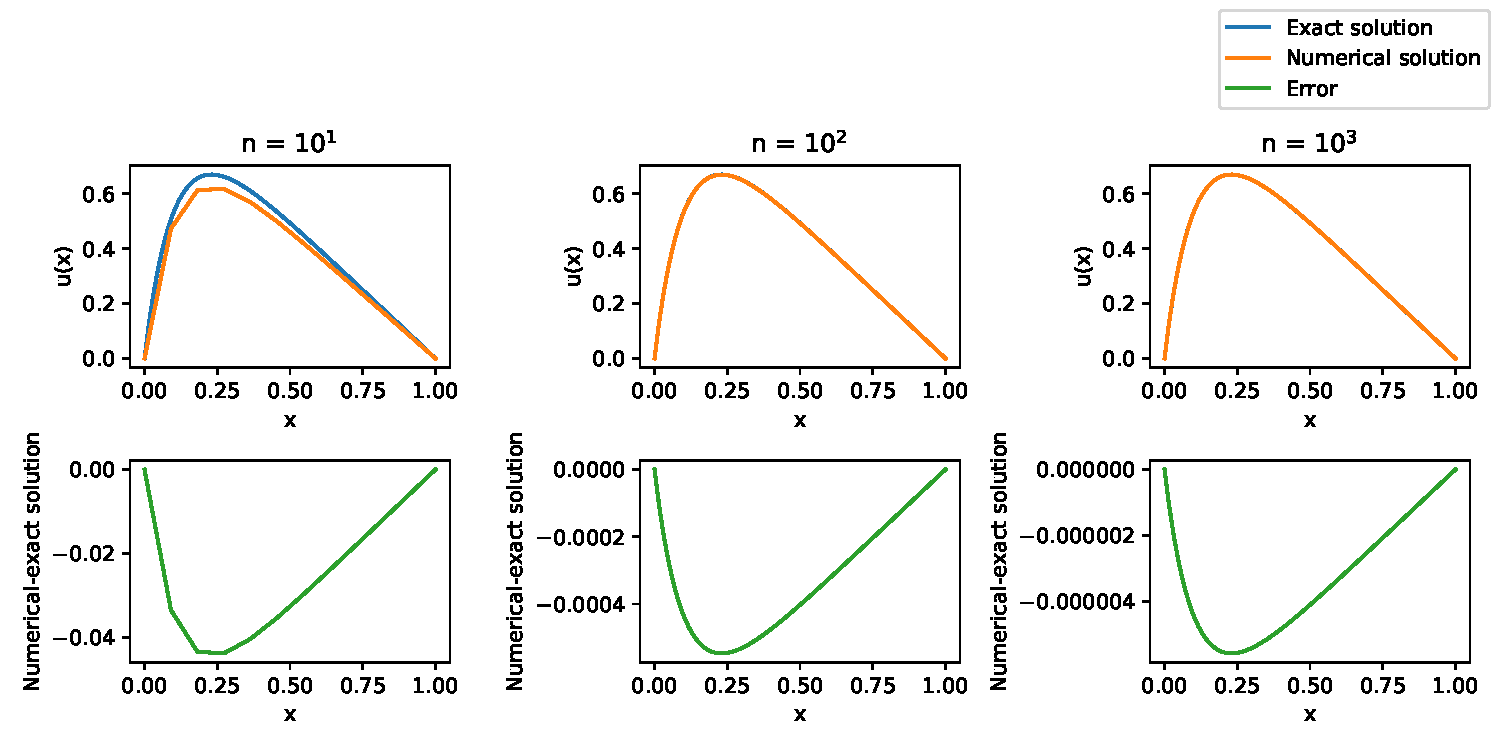
\includegraphics[width=0.96\linewidth]{general_plot.pdf}
  \caption{Numerical solution (from the general tridiagonal matrix algorithm) for $n=1$, $n=10$ and $n=1000$, compared to the exact solution.}
  \label{fig:general_plot}
\end{figure}
\begin{table}[ht]
  \centering
  \begin{tabular}{c c c c c c c} \toprule
    & \multicolumn{2}{c}{Tridiagonal (general)} & \multicolumn{2}{c}{Tridiagonal (special)} & \multicolumn{2}{c}{LU decomposition}\\\cmidrule(lr){2-3} \cmidrule(lr){4-5} \cmidrule(lr){6-7}
    $n$ & t [s] & Rel. error & t [s] & Rel. error & t [s] & Rel. error \\\midrule
    10 & $3.94\mathrm{e}{-7}$ & 0.0661 & $2.68\mathrm{e}{-7}$ & 0.0661 & $1.10\mathrm{e}{-4}$ & 0.0661 \\
    $10^2$ & $2.39\mathrm{e}{-6}$ & $8.17\mathrm{e}{-4}$ & $1.65\mathrm{e}{-6}$ & $8.17\mathrm{e}{-4}$ & $6.55\mathrm{e}{-4}$ & $8.17\mathrm{e}{-4}$ \\
    $10^3$ & $2.83\mathrm{e}{-5}$ & $8.32\mathrm{e}{-6}$ & $1.86\mathrm{e}{-5}$ & $8.32\mathrm{e}{-6}$ & 0.0565 & $8.32\mathrm{e}{-6}$ \\
    $10^4$ & $3.78\mathrm{e}{-4}$ & $8.33\mathrm{e}{-8}$ & $2.27\mathrm{e}{-4}$ & $8.33\mathrm{e}{-8}$ & 13.47 & $8.33\mathrm{e}{-8}$ \\
    $10^5$ & $4.78\mathrm{e}{-3}$ & $1.44\mathrm{e}{-9}$ & $2.86\mathrm{e}{-3}$ & $8.33\mathrm{e}{-10}$ & - & - \\
    $10^6$ & 0.0367 & $8.40 \mathrm{e}{-7}$ & 0.0249 & $6.87 \mathrm{e}{-11}$ & - & - \\
    $10^7$ & 0.347 & $2.98 \mathrm{e}{-6}$ & 0.214 & $8.13 \mathrm{e}{-10}$ & - & - \\\bottomrule
  \end{tabular}
  \caption{Comparison of the CPU time used (averaged from 10 runs) and the maximum relative error for the general and specialized tridiagonal matrix algorithms, and the general LU decomposition method, for various numbers of integration points $n+2$.}
  \label{tab:mainresults}
\end{table}
\subsection{Round-off errors}
The errors in table \ref{tab:mainresults} also agree with the previous discussion; for small $n$ the errors are identical, i.e. all methods give the same results, however as $n$ grows large the specialized tridiagonal algorithm gives significantly more precise results. This is, as  I discussed in the previous section, due to the fact that in the specialized version all the $\tilde{b}_i$'s are calculated exactly, before the main part of the algorithm, whereas in the general version they are calculated in the main part of the algorithm, by repeated subtractions. When this process is repeated a very large number of times small round-off errors in the values of $\tilde{b}_i$ can begin to add up, which by extension leads to errors in the solution. \par
The sizes of the errors for small $n$ also behave as expected from the approximation for the second derivative I used; the leading term of the error in equation \ref{eq:2ndderivative} is of order $h^2$\cite{lecturenotes} ($h=1/\left(n+1\right)$), and one can indeed see that for small $n$ the maximum relative error increases roughly by a factor $100$ every time $n$ increases by a factor of 10. However as $n$ grows larger this trend stops, and the error starts to rise again. To examine this further I compared the logarithm of the maximum relative error (i.e. the maximum value of $\epsilon_i = \log_{10}{\norm{\left(u^*_i-u_i\right)/u_i}}$) to the logarithm of $h$, for the specialized tridiagonal algorithm. The results are shown in table \ref{tab:error_tab} and figure \ref{fig:error_plot}. \par
\begin{table}[ht]
  \centering
  \begin{tabular}{c c} \toprule
    $\log_{10}{\left(h\right)}$ & $\epsilon$ \\\midrule
    -1.0414 & -1.1797 \\
    -2.0043 & -3.0880 \\
    -3.0004 & -5.0801 \\
    -4.0000 & -7.0793 \\
    -5.0000 & -9.0791 \\
    -6.0000 & -10.1628 \\
    -7.0000 & -9.0900\\\bottomrule
  \end{tabular}
  \caption{$\epsilon \equiv \text{max}\left(\epsilon_i\right)$ (maximum value of the logarithm of the relative error from the specialized tridiagonal algorithm) vs the logarithm of the step size $h$.}
  \label{tab:error_tab}
\end{table}
\begin{figure}[ht]
  \centering
  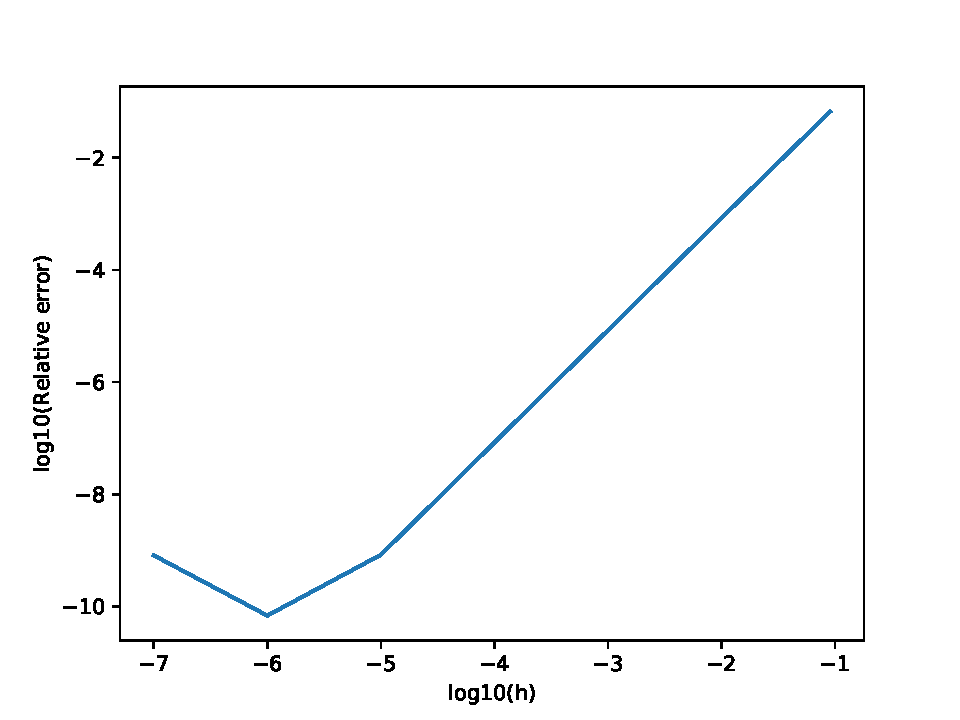
\includegraphics[width=0.84\linewidth]{error_plot.pdf}
  \caption{$\epsilon \equiv \text{max}\left(\epsilon_i\right)$ (maximum value of the logarithm of the relative error from the specialized tridiagonal algorithm) plotted against the logarithm of the step size $h$.}
  \label{fig:error_plot}
\end{figure}
These results show that the logarithm of the relative error is indeed linear with respect to the logarithm of the step size, with a slope of 2, for relatively large $h$. As $h$ gets smaller, however, the error starts to increase. This happens because of round-off error; as the number of integration points increases the difference between the elements of the vector $\vec{g}$, and between those of $\tilde{\vec{g}}$, become very small. When floating point operations are performed on these (especially subtraction - the difference between two values is given by a small number of significant digits - but this does not occur in this case) small round-off errors can easily arise, and when a very large number of such operations are performed these errors can add up and become significant. As was seen in table \ref{tab:mainresults}, this effect is more apparent for the other solution methods, which as I discussed earlier is because the effect of round-off errors adding up also affects the values of $\tilde{\vec{b}}$ in those methods.
\section{Conclusions}
From the results presented here one can see that when solving Poisson's equation numerically, the specialized version of the tridiagonal matrix algorithm is clearly preferrable over the general version, and LU decomposition, as it is both faster (although the difference between the two tridiagonal matrix algorithms is rather small here, as both have CPU times proportional to the number of integration points) and more precise. This is hardly surprising; an algorithm which is specialized to a particular problem should perform better than general methods for that problem. This does not mean that the more general methods are useless, however; if one has to solve many different sets of matrix equations it might be simpler to use some general algorithm (the general version of the tridiagonal matrix algorithm if the matrices are known to be tridiagonal; if not, LU decomposition is better suited) for all of them rather than developing a specific algorithm for each case. \par
I have also demonstrated the effect of round-off errors as the number of integration points increases; initially, when decreasing the step size, the relative error is proportional to the step size squared as one would expect from the form of the approximation of the second derivative given in equation \ref{eq:2ndderivative}. However, when the number of integration points grows very large round-off errors can become significant. This shows that when solving differential equations numerically one cannot blindly keep reducing the step size in the hope that the error will keep decreasing according to the order of the approximation used; round-off errors for small step sizes have to be taken into account.

\begin{thebibliography}{}
  \bibitem{assignment}
    Assignment text for project 1 in FYS3150/FYS4150,
    Department of Physics, University of Oslo, Norway

  \bibitem{lecturenotes}
    Hjorth-Jensen, Morten,
    2015,
    Computational Physics - lecture notes

  \bibitem{LUslides}
    Hjorth-Jensen, Morten,
    2018,
    Computational Physics Lectures: Linear Algebra methods
  \bibitem{armadillo1}
    Sanderson, Conrad and Curtin, Ryan,
    Armadillo: a template-based C++ library for linear algebra,
    Journal of Open Source Software, Vol. 1, pp. 26, 2016

  \bibitem{armadillo2}
    Sanderson, Conrad and Curtin, Ryan,
    Practical Sparse Matrices in C++ with Hybrid Storage and Template-Based Expression Optimisation,
    Mathematical and Computational Applications, Vol. 24, No. 3, 2019
\end{thebibliography}
\end{document}
